\chapter{Antecedents of Modern Urban Rent Theory: Rent and Production} \label{chapter-rent}
% MOVE - Land rent was historically the basis of the wealth and political power of  the land-owning class in the era of the classical economists. % ***E NEED MORE HERE

\epigraph{Of the concrete forms of income that have usually been classed as surplus, the rent of land was the earliest to be defined; and so prominent a position has been given to it that the terms ``rent'' and ``surplus'' have come to be used interchangeably.}{Alvin Saunders Johnson, 1902 \cite{johnsonRentModernEconomic1902}}
\epigraph{The law of rent has become an obstacle to scientific progress: it has retarded the attainment of a true theory of distribution ... %Yet it is itself capable of affording such a theory. 
The principle that has been made to govern the income derived from land actually governs those derived from capital and from labor. 
}{John Bates Clark 1891 \cite{clarkDistributionDeterminedLaw1891}}

% for those with financial assets.
Financialization is the capture of surplus. Rent is key to how economists have studied the distribution of the surplus. % It was central in classical economics.
% In order to model what's happening in financialization, we need the concept of rent. https://www.overleaf.com/project/606a6b286ae1c9f203fadab5
% In 1902 Alvin Saunders Johnson \cite{johnsonRentModernEconomic1902} summarized the relationship between rent and surplus in the economic literature as follows: 
% \begin{quotation}Of the concrete forms of income that have usually been classed as surplus, the rent of land was the earliest to be defined; and so prominent a position has been given to it that the terms ''rent'' and ''surplus'' have come to be used interchangeaby.\end{quotation} 
\Gls{rent}, in economic theory is not the amount a tenant pays a landlord every month, nor is it simply a payment for using land or another facility.  For economists, the word normally means the \gls{surplus} income produced by a scarce factor of production that is created by nature. People pay a high price for housing near the center of a city because there is limited %nature did not make much
land close to the city center and having people close to urban jobs and amenities is valuable. The extra cost to be close to the center is an \gls{economic rent}. It was not created by the landlord, but it appears as income for the landlord. Thus the economist's notion overlaps with, but is not identical to the common usage. 

In this thesis, we identify what are essentially \glspl{classical rent} in the urban system and examine their distribution to develop a model of financialization of the urban housing market.
If financialization is capturing the stream of \glspl{locational rent}, that is the stream of \glspl{surplus}, we need to understand theories about who captures surpluses how, and this leads to classical and neoclassical economics and the theories of rent and production.

In this chapter, we build a bridge from \gls{classical rent theory} to the modern theory of urban rent, which this thesis works to develop. 
To do this, we trace the development of antecedents to the work on modern urban rent theory develop in this thesis, beginning with classical tradition of rent, and tracing through the development of the neoclassical tradition, and modern theories of production. 
% We bring in the concept of rent because it is necessary background for our examination of the impact of \gls{financialization} on urban productivity. 

% ***E NEED TO EXPLAIN THIS MORE BEFORE MOVING TO THE NEXT SENTENCE. DRAW OUT THE DEFINITION SO IT'S REALLY CLEAR.  

% ***E OR MAYBE OPEN WITH THIS? OR: Economics is the study of ___. It is concerned with production (i.e. ___ and distribution (ie. ___) 

% We use the \gls{Cobb-Douglas} function %, which is used to cross this entire range of literature to illustrate each link and to show how our model is directly connected with this broad collection of linked theories. 
% The \gls{Cobb-Douglas} function is a production function, expressing the output produced, in terms of inputs such as labour and capital.
% Our model connects to the results in this chapter at four points:

% In the following chapters we will discuss the three pieces of theory needed to build a model of financialization, rent, urban spatial models, and growth theories. From there, we will bring these things together into a formal model in Part \ref{part-model}.
 
\section{Classical theories of production, distribution, and class}
Classical Rent theory originates with  thinkers such as Richard Cantillon (1680s-1734), 
Fran\c{c}ois Quesnay (1694–1774), the marquis de Mirabeau (1715–1789), Anne-Robert-Jacques
Turgot (1727--1781) and 
Adam Smith (1723-1790), and received its classic statement
in Ricardo (1772-1823). Nearly contemporaneous thinker, 
Johann Heinrich von Th\"unen (1783-1850) developed a planning model to guide the location of economic activities for an urban-agricultural society. A version of that model was reinvented in urban geography by William Alonzo.

The canonical presentation of the classical theory of rent \cite{ricardoEssayInfluenceLow1815} was provided by David Ricardo in 1815 in the context of a primarily agricultural economic system during increasing globalization of trade and the early stages of the industrial revolution in Northern Europe.\footnote{The Industrial Revolution is usually described as beginning around 1760 and having significantly transformed society by about 1820–1840.} In this period, the study of \gls{political economy} was emerging as a subject of study that focused on understanding trade, wealth, and government.\footnote{Prior to this, international relationships centred on studies of the military. As colonization changed the relationship between countries and trade became central, the study of \gls{political economy} became more significant}

For the economists of the very early stage of the industrial revolution, % it seemed clear that 
all wealth came from the land. Trades people, professionals, clergy, and aristocrats were %all 
nonproductive.\footnote{The Physiocrats in particular, a school of economists in 18th-century France, emphasized  that land is the source of all wealth, that only agricultural labour was productive, and that government policy should not interfere with the operation of natural economic laws. With this framework, they were the first to frame labour as the source of value. Marx generalized this analysis, treating industrial labour as generating a surplus as well.}

% Looking more closely they could see that
They noted that only some land produces a surplus of income. Good land produced more market value for the same cost as the poorest land in production. The poorest land in production just barely justified the cost of production. After paying for labour and any other costs of production there was no surplus left for the land owner. More fertile land generated more than the annual costs faced by a landowner. 

The difference in earnings between the poorest land in production and a more fertile or better located field was the quantity that economists called rent. In the classical tradition, rent is the surplus produced by labour using land that is claimed by landowners by virtue of their ownership of the land. Ricardo defines rent strictly in this way, saying ``By rent I always mean the remuneration given to the landlord for the use of the original power of the land.''\cite{ricardoEssayInfluenceLow1815} The key term in that definition is ``the original power of the land.'' The price of the corn would include payment for working the land and for transporting, storing, and  selling the product, but the part that was rent would be a payment for the virtue of the land not of the landlord. % ***E CLARIFY THIS SENTENCE. 
  
 Economic rent and the rent paid by farmers to use the land were almost interchangable concepts. Landowners would generally not %prefer not to 
 till the soil or bundle sheaves themselves. They would `rent out' the land. The level of rent charged might not be exactly the economic rent, but in a labour-surplus economy\footnote{Between 1604 and 1914 over 5,200 enclosure Bills were enacted by Parliament which related to just over a fifth of the total area of England, amounting to some 6.8 million acres. From the 1750s enclosure by parliamentary Act became the norm. In Scotland  between 1750 to 1860 the  Highland Clearances  evicted a significant number of tenants in the Scottish Highlands and Islands, mostly in two phases from 1750 to 1860. Enclosures and clearances created a large pool of essentially minimum wage labour that supported industrialization and drove British migrations to the colonies.} landlords had a great deal of bargaining power, and the rents they charged their tenant farmers tended to approximate the value of the surplus. Rent as a price and economic rent would have been close. % practically the same.
 \footnote{The social question that Ricardo answered was: who gets the surplus generated by the land after all other contributors have been paid. This was an approach to understanding the distribution of wealth and explaining the inequality the economists were seeing. 
 
 For Ricardo this theory provided insight into whether Britain should open its doors to corn from the colonies. This was the debate over the Corn Laws (1794-1846), a set duties on grain imports into Britain to protect British agriculture from outside competition. In Britain, ``corn'' was the generic name for cereal crops. The full title of Ricardo's essay was was \textit{An Essay on the Influence of a low Price of Corn on the Profits of Stock, showing the Inexpediency of Restrictions on Importation: With Remarks on Mr Malthus' Two Last Publications: "An Inquiry into the Nature and Progress of Rent," and "The Grounds of an Opinion on the Policy of restricting the Importation of Foreign Corn"}.
His model  explained the distribution of the product of the earth among the “three classes of the community” which is to say, to the owners of land, labour, and capital.   %EXPLAIN SHIFTS  ACCORDING TO HIS ANALYSIS .. 
The economic transformations of the period resulted in an increase in overall wealth, although in many cases the living condition of the working class declined.} % THIS IS WHAT RICARDO AND OTHER CLASSICAL ECONOMISTS WERE CONCERNED WITH EXPLORING}

 % This is what Ricardo developed the concept of rent to explain.  
 % \Gls{class} structure, or how different classes participate in production changes over time as modes of production change. When Ricardo was writing, the economy was still largely reflected feudal social relations in that most land ownership originated in feudal military power. %Even the land of the nobility was divided up into smaller parcels run by knights or vassals. Both of these groups traded military support for land in the local manors. As higher ranking people, knights often presided over an entire manor, while vassals presided only over the land needed to support their families.
 % (IE DESCRIBE role of labour land, capital under feudalism and how this was changing in that period.) 
 
% ADD The evolution of the mode of production has continued, with human capital rather than land or industrial capital increasing the source of the social surplus. The concept of rent is specifically relate to surplus and enabled Ricardo to first talk about how is key to distribution within the economy, amongst classes.  Ricardo essentially developed his concept of Rent to explain the dynamics of distribution between classes. 

% ***E i LIKE THIS STUFF ABOUT THE PHYSIOCRTAIC SCHOOL. YOU MIGHT MORE DIRECTLY FRAME IT IN THE CONTEXT OF A BROADER QUESTION OF VALUE, ROLE IN PRODUCTION AND DISTRIBUTION OF SURPLUS. 
% going back to the Physiocrates. 
% The physiocratic school of economics was the first to see labour as the sole source of value but, for the physiocrats, in the context of the prevalent European rural society of the time, only agricultural labour created a surplus. % actually? % detail for it was ag economy This was the theory? also the french engineers- detail for start of math/calc-..
%The canonical reference for only agricultural labour mattering? For the definition of rent?

For Ricardo, and for the classical economics in general, land rent, is thus a kind of surplus value, that is an amount available after the costs of production have been paid, the term rent came to be used interchangeably with this more general concept in much of the classical work on rent and the term rent has been used in a more general sense to other kinds of surplus value, as well as land rents. 
Surplus value is essentially profit. Its the value beyond the cost. 
 
% ***E COULD ADD HERE IF YOU HAVEN'T ELSEWHERE... MAYBE ADD:
%(
% It's easy enough to see how this concept would evolve into the two different usages of the term rent. Because it is the profit for the land, which is related to payments for the land. At the time, the feudal ownership structures meant that the value of the land was structured differently. Tenants did not pay to occupy the land the way that people and businesses do today. Rather the value of owning land was reflected in the distribution from production. The term later split to reflect both the way land is currently valued (i.e rent payments to occupy) and the surplus value that was how land was valued in the period of clssical econmics with it's feadul structures. Rent became payment to landlord because under feudalism, the surplus went to the landlords. Thenn the term diverged into the two distinct meanings used colloquially and in a technical context by Economists ) 






%The profit now accrues to the landowner, and we call it land rent. For Ricardo, it was obvious that the land-owning class captured the land rent.

\subsection{Rent, space, and profit in agricultural markets}

% who picks up vegetables at the farm gate, transports them into town, and sells them to a storekeeper. He pays the farmer at one end of the trip and is paid at the other. 
Rent  can be illustrated with the story of a carter, who purchases produce, say potatoes, from farms, and carries them, on a cart, to sell in town.
% Imagine an  town in Ricardo's context, surrounded by potato farms, with people who pulled carts to carry potatoes to sell at a market. 
% Imagine there is one person who owns the only cart in the region that can be used to move potatoes. Now imagine that this monopoly carter notices that 
There is a price for potatoes in town and a lower price at the farm gate, so the carter can buy potatoes from farmers, carry them to market and resell at a higher price in town. What remains of the price gap after subtracting labour and vehicle costs, is profit.  

\begin{figure}[htb]
    \begin{center}
     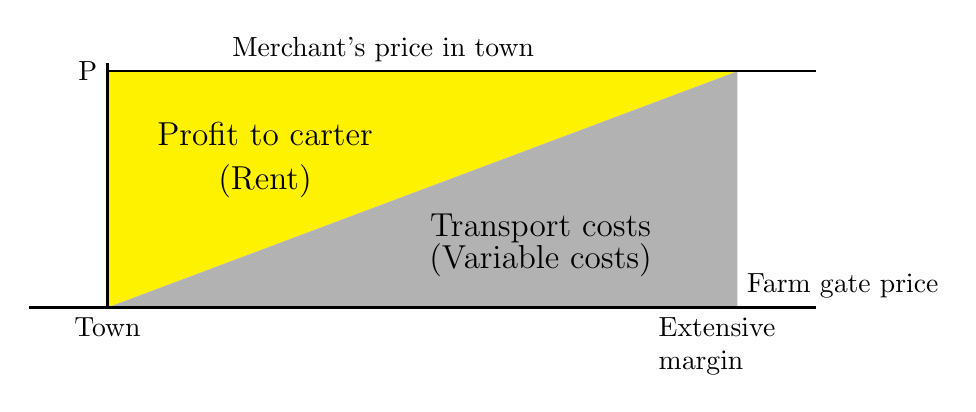
\begin{tikzpicture}[domain=0:2]
%\draw[thick,color=gray,step=.5cm, dashed] (-0.5,-.5) grid (3,3);
%\draw[line width=.01, green ] (0,0) -- (10,0) node[right  ] {Distance};
\node at (1,0) [below] {Town};
\fill[yellow]  (1,0) --(9,3)--(1,3) --cycle;
\fill[gray!60] (9,3) --(1,0)--(9,0) --cycle;

\draw[thick ] (1,3)node[left]{P}  -- (10,3);\node at (4.5,3)[above ] {Merchant's price in town} ;
\draw[thick ] (0,0)  -- (10,0); 

%\draw[thick,color=red] (1.5,0) -- (1.5,1) node[below right] {Fixed cost} -- (1.5,1.5) --(10,3.25)node[above left] {total cost};
\draw[thick] (1,0) -- (1,3.1) ;
\node[below,text width=2cm]at (9,0) {Extensive margin};
%\draw[ultra thick, blue,<-> ] (3,1.8) -- (3,2.5)node[left] {annual rent at a} -- (3,3) ; 
\node at (9,0)[above right] {Farm gate price};
\node  at (6.5,1){\large Transport costs};
\node  at (6.5,.6){\large (Variable costs)};
\node  at (3.,2.2){\large Profit to carter};
\node  at (3.,1.6){\large (Rent)};
\end{tikzpicture} 
    \caption[Ricardo's theory of extensive margin.]{Ricardo's theory of the extensive margin using transportation costs to emphasize the similarity between rent in classical theory and in the Alonzo model, developed in the next chapter, Chapter \ref{chapter-space}. Transport costs, the yellow area, take a share of the profit for vegetables sold in the town}
    \label{fig-rent-ricardo}
    \end{center}
\end{figure}

Beyond certain distance, the costs of the trip will eat up all the profits. That is the farthest distance the carter will go to buy potatoes. That distance is Ricardo's \gls{extensive margin}.\footnote{Ricardo carefully distinguished the \gls{intensive margin} and the \gls{extensive margin}. The extensive margin is where the most distant land worth cultivating given the cost of transportation. The intensive margin, on the other hand, can be seen as the limit to increasing the productivity  of a particular piece of land by applying fertilizer, draining, or paying more workers. It's the improvements available.} % The extensive margin provides a key insight  into modern urban tent theory. 
ELABORATE ON WHY EXTENSIVE MARGIN MATTERS. - QQQ FERTILITY VS DISTANCE TO MARKET\footnote{In most of the discussion Ricardo emphasized  differential land fertility rather than distance to market.}
Figure \ref{fig-rent-ricardo}, shows the total transport costs as the yellow area. The area below the yellow triangle is profit for the carter. The carter makes a `profit' on the trip to the farm nearest to town, a lower profit farther from town, and no profit on any farms beyond this point.\footnote{Note the similarity with Alonzo's urban model, illustrated in Fig \ref{fig-rent-alonzo}.}

Together these two triangles/areas represent the net farm-gate value of the ``produce of the earth'', but only the lower triangle is surplus that can be allocated to the landlord, the carter, the merchant or the consumer.\footnote{It was termed the `\textit{produit net}' by the Physiocrats} In modern supply and demand analysis it would be recognized as `producer surplus', the difference between what a producer gets for a good and what they would be willing to accept.

We have illustrated the story using a carter with a monopoly on transportation services. If instead there were a monopoly landowner, and the transportation industry were competitive, the landowner would pay carters and farmer workers their minimum cost and keep the profit. In this case economists would call the monopoly profits rents. %\footnote{In the modern economy, agricultural land rents may be captured by corporations,  either by owning the land or by controlling the supply chain.}  
Landlord income in this example is a locational \gls{land rent} that exists because of the land's proximity to the market.  
% ***E ADD?? This graph is simplified to illustrate the concept.
(TODO note how this formalizes power as an  emergent phenomena, with particular hysteresis properties, and distributional characteristics. Power is both formally representable and directional, almost in a gauge like sense.)

The land rent %(that was profit) 
declines with distance from the town.\footnote{It also declines for less fertile land, where there is a higher cost of production.} 
At the extensive margin, land rent falls to zero. Even fertile land beyond the extensive margin will not be farmed because the product cannot be transported to market at a profit. Transportation costs and the price of produce in town determine the size of the  rent triangle, and the amount of rent captured by the land-owning class.%\footnote{The debate about the  `Corn Laws" that Ricardo  was engaged in was about whether Britain would allow wheat from Canada and Australia to enter, reducing the price of wheat and therefore reducing the income and influence of the land-owning class.} 

If the merchant's price went up, the \gls{extensive margin} would move farther out, and more land would come into production.\footnote{This simple example assumes that the land is uniformly productive and that there is only one product that can be marketed. Johann Heinrich von Th\"unen, in The Isolated state (Der isolierte Staat (1826)\cite{vonthunenIsolirteStaatBeziehung1826}), provided a more complex analysis based on the same principles.}
% For simplicity, assume all farmers have the same cost of production, and the carters pay the farmer the farm gate price at the farm and receive the merchant price in town. 


\section{Two stories of distribution}
There is a long history of economists thinking about the distribution of the surplus. %, going back to the early work in classical economics and continuing through Neo-classical economics. 
There are two dominant theories of \gls{distribution} in economics. The first and oldest is based on the classical concept of rent as explained  by David Ricardo \cite{ricardoEssayInfluenceLow1815}, in which owners of land are able to extract a value beyond what they contribute based on their ownership of a scarce resource. The second is the marginalist approach, developed by John Bates Clark and others, in which workers and other factors  in competitive markets receive the \gls{marginal value-product} of their contribution to production. The two theories coexist and even mingle in modern economics, but it is the marginalist approach that dominates economic teaching. 

Both theories developed in response to the social and economic conditions of the periods in which they emerged. Both attempt to explain where the output of society ends up within society. They are, at their heart, stories of who %can or does 
claims what share of production. Classical rent theory emphasized the distribution of the social \gls{surplus}, the part of production over and above what was needed to reproduce society. Initially this included only land rents, but was later extended by Marx to the distribution of profits.
The classical theory of rent was the foundation of early %the first satisfactory theory 
theories of income distribution. It linked a spatially distributed economy, agriculture, with the class structure of the society of the time. 

The distribution of these surplus incomes are not explained by the later neoclassical theory. In fact they are assumed to be a transitory phenomenon that disappears as a result of free competitive market entry, even though profits and rents remain a substantial part of national income (20–25 percent) \cite{GET_Britannica} %\footnote{Schmitt, Hans Otto, Pen, Jan, Boulding, Kenneth E. and Kleinsorge, Paul Lincoln. "distribution theory". Encyclopedia \cite{GET_Britannica},  \url{https://www.britannica.com/topic/distribution-theory}. Accessed 22 February 2023.} 
in the world the neoclassical model describes. 


% To build a model of financialization, we need to bring in a concept of rent, that was central in classical economics, but has not been as important in formal neoclassical modeling.
% which is described in the next chapter and to which this thesis contributes. 
% We trace the development of theories of income distribution through the classical and neoclassical periods to provide context to our contribution to the development of a modern urban rent theory.  
% We correct that omission because they are
% Along the way, we also explain how the competing approach to distribution, has perhaps unintentionally left most

We contribute to a modern theory centered on human capacity.

% MODE OF PRODUCTION

% STATE OF THE WORLD

% METHODOLOGICAL FRONTIER

\subsection{A changing economy brought a change in the theory of distribution}
As the economy shifted  moved from overwhelmingly  agricultural into the industrialization of the 18$^{th}$  and 19$^{th}$ century, economists shifted their focus from who got the rents to how prices and especially the prices of factors of production were determined. Rent theory was eclipsed by an approach that focused on the markets for the inputs used in industrial production.  Late in the 20$^{th}$ century, the focus shifted again, to the economics of  knowledge, human capital, and how cities generate wealth, a change that plays a part in  our theory of urban rents in Chapter \ref{chapter-growth}. 
 
The changes have tracked changing social relations. The influence of landowners declined and the power of  industrial capitalists increased throughout the 19$^{th}$ century. More recently the owners of industrial capital have been eclipsed, to some extent, by financial capital and by the owners or creators of certain information technologies.


\subsection{Rent and industrial capital}

Early theories of rent and industrial production centered rent in the classical sense.

MARX IS LINK TO INDUSTRIAL CAPITALISM
EARLY THEORIES OF INDUSTRIAL CAPITALISM ACTUALLY STILL CENTERED RENT, IT WAS THE NATURAL WAY TO UNDERSTAND THIS. SEE MARX, HENRY GEORGE EXTENSION TO THE CITY.
There was a shift to industrial capitalism from an agricultural economy.

There were some efforts to integrate rent in the analysis this new economic reality, like that by Marx. 
It was eventually displaced in the neoclassical work of thinkers like John Bates Clark.
%Ricardo, agreeing with Malthus, essentially assumes that the wage is  just sufficient to reproduce the labouring class.\footnote{``In the natural advance of society, the wages of labour will have a tendency to fall, as far as they are regulated by supply and demand; for the supply of labourers will continue to increase at the same rate, while the demand for them will increase at a slower rate.''} He then explains the distribution of the fruits of labour on the land among the main classes of the economy.
%***E ADD CONTEXT like:

Marx's work is an example of an analysis of a system level of effects of shifts in structures of financial capital financial instruments, in a sense of a different iteration of financialization of the previously non-financial- but financialization embedded in production. Later stories decoupled from production, with the financial structures coming to run on a logic of their own.

Karl Marx (1818--1883)) was born three years after Ricardo published his Essay on the price of corn. 
By the time Marx was displaying  his developing interest in economics  at the radical newspaper, Rhineland News, Ricardo had been dead 20 years, the industrial revolution had been underway for almost a century and European economies were largely structured around manufacturing. 

 % ***E MORE ACCURATE TO SAY HE was exploring this because it was what he saw than shifted attention.
 In the manufacturing economy, the owners contribute the machinery, buildings, and even working capital to fund the workers until the product can be sold. % ***E FLESH OUT THIS DESCRIPTION OF THE KEY FEATURES OF TEH MANUFACTURING ECONMY. ALOS SPECIFCAL DEFINE CAPITAL CAN WHY IT MATTERS
 %This contribution must be accumulated from their profits in the preceding cycle of production,  and has to be reinvested once the revenues of the current round have come in and the bills have been paid. Marx actually describes a circuit of capital from its form as money to its form as physical capital. 
As in Ricardo, however, labour is in surplus and capital is scarce. As in Ricardo, the scarce factor is owned by a special class - now the capitalists - who are able to appropriate the surplus value. %Like Ricardo,  Marx saw the appropriation of surplus as without moral justification. 

Marx pointed to an additional dynamic feature of  capitalist systems - that productive capital is not fixed as land is, but  expands as surplus is reinvested. This creates an economy that can and, according to Marx, must grow, as well as challenges that are created by the capitalists' need to constantly reinvest their growing accumulation of surplus value. It was not until 1867 that  the first volume of Das Kapital,  was published, pulling together 20 years of Marx's analysis of the capitalist economy.  Das Kapital proposes an explanation of the "laws of motion" of the mode of production from its origins to its future by describing the dynamics of the accumulation of capital. With topics such as the growth of wage labour, the transformation of the workplace, capital accumulation, competition, the banking system, the tendency of the rate of profit to fall, and land-rents.% ***E EXPLAIN WHAT THIS MEANS AND WHY IT MATTERS TO DISTRIBUTION. HOW IS IT DIIFFERENT OR SIMLAR TO WHAT WAS HAPPENING UNDER FEUDALISM? 
%He famously suggested that the expansion will eventually outrun the expansion of demand and the rate of return will fall, leaving capitalists unwilling to invest. % and creating a crisis. 

% ***E FILL OUT CRISIS % WHEN i GET TO HENRY GEORGE AND YOU MAKE THE DISTINCTION BETWEEN HIS VIEW OF WHAT WOULD CAUSE CRISIS AND MARX'S, i AM CONFUSED BECAUSE YOU DON'T FULLY ARTICULATE THE PROBLEM. I THINK THIS IS SOMETHING MISSING HERE, BUT YOU COULD ALSO CHANGE THE LINE IN THE GEORGE SECTION IF THIS IS NOT AS IMPORTANT. TO ADD YOU WOULD JUST NEED TO EXPLAIN HOW THE NEED FOR GROWTH ULTIMATELY CREATES A PROBLEM OR CRISIS. WHY IS DOES IT POSE CHALLENGES. 
%***E I ALSO THINGK THAT THIS LIST OF TOPICS IN THE BOOK IS A BIT OF AN ABRUPT END TO EXPLAINING MARX'S CONTRIBUTIONS. IT WOULD BE HELPFUL TO PAINT MORE OF A PICTURE OF WHAT HE DOES WITH THESE TOPICS. INCLUDING THE CRISIS THING BUT ALSO A BIT MORE GENERALLY. THE TRANSITION TO HOW YOU POSITION MARX IS CURRENTLY A BIT ABRUPT. 


% ADD? We see Marx as firmly part of the Classical tradition and a contributor to distributional theory.  Our work, linking urban rents to the dynamics of financial capital has one foot firmly  in the Ricardian and Marxian  tradition. Like Marx and Ricardo we explore how a particular type of surplus is distributed, how that might change, and the effect on society  ***E OF THE VARIOUS SYSTEMS OF DISTRIBUTION?. Like Marx and Ricardo we find that a functional approach to social classes provides a useful framework. Where Marx focused on industrial \gls{capital}, however, we focus on capital in a different form: \gls{financial capital}% ***E SEEMS TO BE A LOT MISSING HERE?

% ***E i FEEL LIKE IT WOULD BE USEFUL TO DESCRIBE THE CLASS BREAKDOWN IN MARX AS IT RELATES TO HOW THE DIFFERENT ROLES FIT INTO PRODUCTION. aLSO. WHAT HAPPENED TO THE IDEA OF LAND RENT IN THIS PERIOD AND IN MARX'S WORK SPECIFICALLY? dID HE IGNORE IT? EVEN IF HE DIDN'T USE THE CONCEPT, EXPLAIN HOW IT WOULD RELATE OR FIT (OR NOT FIT) INTO THIS CONCEPT)

\subsection{Henry George, rent and cities} 

As Marx linked rent and industrial produciton, Henry George linked rent and cities
% In economics Henry George's work links rents and space
, but it has not been taken up to the degree that it could be. 
% ***E THIS SECTION FEELS A LITTLE SPARSE ON ECONOMIC ANALYSIS %YOU EXPLAIN GEORGE'S CONCLUSIONS VERY CLEARLY, BUT I FEEL THIS WOULD BE STREGTHEN A LITTLE MORE CLARITY ABOUT HOW HE RE-INTRODUCE LAND RENT. WHAT WAS THE ANALYSIS / iNSIGHT EXACTLY? THEN GO INTO THE CONCLUSIONS HE DREW ABOUT WHAT SHOULD HAPPEN...
In 1879, Henry George (1839--1897), an influential American political economist, published his most famous work, Progress and Poverty\cite{georgeProgressPovertyInquiry1973}. It sold millions of copies worldwide. George returned to land rent with a new insight based on the emergence of the capitalist city: the owners of urban land extract surplus in exactly the same way that owners of agricultural land do in Ricardo's analysis. ``With the growth of population, land grows in value, and the men who work it must pay more for the privilege.''  Where Marx saw the extravagant productivity of capital as the source of capitalist crises, George saw the extraction of wealth by land speculators as the mechanism that would bring on crises.
  % ***E WHAT DID HE MEAN BY CRISIS? HOW DID HE COME TO BE CONCERNED ABOUT THIS? ALSO SINCE YOU ARE COMPARING WITH MARX's PREDICTIONS ABOUT CRISIS YOU NEED TO EXPLAIN MORE ABOUT MARX'S IDEAS OF CRISIS ABOVE
  % ***E Somewhere in HERE YOU MAY WANTED TO EXPLAIN SOCIALISM VS MARXISM... GEORGE IS SOCIALIST? MARX?? PUTTING IN THE CONTEXT OF HOW THOSE TRADITIONS WERE EMERGING MIGHT BE HELPFUL... I HAD THIS NOTE ON THE PAPER DRAFT... COULDN'T FIGURE OUT WHY SINCE YOU DON'T SAY GEORGE IS A SOCIALIST. bUT YOU DO LATER WHEN YOU EXPLAIN THE SHIFTS IN jb CLARK'S THINKING. IF YOU WANT TO CONTEXTUALIZE CLARK IN TERMS OF SOCIALISM ... BEST TO MAKE SURE YOU'VE EXPLAINED THAT GEORGE IS A SOCIALIST, WHAT THAT MEANS, AND THEN, SINCE MARX IS FAMOUSLY BUT CONFUSINGLY INTERCONNECTED WITH SOCIALISM YOU SHOULD EXPLAIN HOW HIS THINK AND (SEPARATELY) THE MOVEMENT NAMED AFTER HIM FIT IN) 
  % # ADD George also presented solutions to ____ 
  
Since land rent is not created by its owners, George argued that land rent should be seen as a social income - that it could be used to pay for all the needs of the community. The clearest statement of this view is found in Progress and Poverty when he wrote "We must make land common property." The same view was expressed by the Physiocrats who concluded  that ``ground rents'' should be the source of most or all taxes. They defined ground rent as that portion of all rent which is attributable only to the size and location of the parcel. George's analysis the `single tax' movement, which sought to shift all taxation to land  and resource rents.   
  
In 1977, Joseph Stiglitz, using Alonzo's relatively new urban model, identified the conditions in which Henry George's "single tax" is  the only tax necessary to finance public expenditures.\footnote{Arnott, Richard J.; Joseph E. Stiglitz (November 1979). "Aggregate Land Rents, Expenditure on Public Goods, and Optimal City Size" (PDF). Quarterly Journal of Economics. 93 (4): 471–500. doi:10.2307/1884466. JSTOR 1884466. S2CID 53374401 }   The logic is fairly simple: if the public good increases productivity or the attractiveness of a city, attracting more people or businesses, land rents rise, and investment in the public good should proceed until the marginal cost of the public good is equal to the increase in land rent it brings. The result is now called the `Henry George theorem.'***E RELATE THIS TO YOUR THESIS. %I FEEL A BIT LOST IN WHAT YOU ARE SETTING UP HERE. COULD YO EXPLAIN HOW THEIS IS RELEVANT TO MODERN URBAN RENT THEORY? 
  
  % ***E MAYBE MOVE UP THIS FOLLOWING PARAGRAPH? %THIS FEELS LIKE IT WOULD FIT WITH MORE DETAILED DESCRIPTION OF HIS ANALYSIS THAT I THINK SHOULD COME BEFORE HIS IDEAS ABOUT THE TAX. 
The classical economists agreed that rents are unearned income. They did not emphasize, as George did, that land rents arise from labour's proximity to urban population and production.\footnote{To be fair, it was not lack of understanding, that the omission reveals, but rather lack of interest in explicitly examining urban land rent from residential or even industrial purposes.}% Ricardo von Thunen, Marx, Cantillon all grasped the notion of proximity to the market as part of the source land rent. The discussions seem to not gone farther than discussions of diffeerential and rents, however.  I just am not aware of them explicitly examining urban land rent for residential or even industrial purposes. 

%The need to be near a market or prodduction center is easily seen by considering a population at the carrying capacity of the land with individuals supporting themselves using purely local resources. There can be no land rent in this case. If a city rises that must be supplied from those still on the land, land close enough to the city will generate land rent. The value of the land is created by proximity to the city.



%  no separate and comprehensive data are provided on the amounts of land rents and subsoil rents charged and earned, because they are not officially regarded as part of value-added, and consequently are not included in the calculation of GDP (except for the value of productive lease contracts)     https://en.wikipedia.org/wiki/Differential_and_absolute_ground_rent#Rent_in_macro-economics    \href{https://en.wikipedia.org/wiki/Differential_and_absolute_ground_rent#Rent_in_macro-economics}{Wikipediat article on differential rent}


\section{Neoclassical distribution theory}
  % # NEED SOME MORE CONTEXT HERE. maybe atart by setting up the PERIOD WE ARE NOW MOVING INTO AND WHAT HAS SHIFTED IN THE ECONOMIC STRUCTURE? 

Classical theories of distribution showed that ownership of a scarce and non-produced factor, land, was the  basis of rent extraction by the class of landowners. Profits were a bit puzzling for the classical economist because their connection to land rents was not as clear. Were profits just a part of land productivity captured by industrial producers as the earliest classical theorists argued, or were they  additional social surplus as the later Classical theorists thought? % ***E i DON'T UNDERSTAND WHY PROFITS ARE PUZZLING? WHATS THE QUESTION? eXPLAIN MORE. update: I STILL DON;T UNDERSTAND.

Alfred Marshall (1842--1924)  one of the most influential economists of his time, and one of the founders of the school of neoclassical economics pointed out that, in a competitive market with free entry, scarcity profits (i.e., rent for capital) would normally be competed away  as entrepreneurs entered the market in pursuit of those `excess' profits. He used the term `quasi-rents' for these unearned but temporary incomes.\footnote{Alvin Saunders Johnson. Rent in Modern Economic Theory: An Essay in Distribution. AEA 3rd Series, Vol. 3, No. 4 (Nov., 1902), pp. 1-129 (129 pages)} This insight suggests that excess profit (profit over and above the normal rate of return on capital) unimportant in the long run, but left it an important short-run role in attracting existing capital to projects where it is most productive.\footnote{Contradicting Marshall, Carey and Lachim \cite{careySomethingNothingHow2019} observe that,``The persistent and growing profit share across a range of advanced economies and within industries fundamentally challenges the assumption of perfect competition and suggests that growing market power is at the heart of many of the economic challenges in America today.''} 

As industrial production grew and eventually exceeded agricultural output..
% {\color{red}
%Adam Smith 
% A monopoly granted either to an individual or to a trading company has the same effect as a secret.… The monopolists, by keeping the market constantly under-stocked … sell their commodities much above the natural price … the price of free competition.…
% The exclusive privilege of corporations, statutes of and apprenticeship, and all those laws which restrain, in particular employments, the competition to a smaller number than might go into them, have the same tendency, though in a less degree. They are a sort of enlarged monopolies, and may frequently … in whole classes of employments keep up the market price of particular commodities above the natural price.… Such enhancements of the market price may last as long as the regulations of police which give occasion to them. wealth of nations
% }
John Bates Clark (1847--1938) was another of the pioneers of neoclassical theory and was one of inventors of the neoclassical theory of  distribution.  The neoclassical or marginalist approach emphasized that rational economic agents pay workers according to the value of the marginal product, the amount that the last worker hired added to output. % ***E DEFINE MARGINAL PRODUCT
The same principle applied to other factors  
Initially a socialist like George,   % ***E YOU NEED TO HAVE SAID ABOVE GEORGE IS A SOCIALIST OR CUT THIS. 
by 1986 Clark was praising the dynamical process of competition and opposing the single tax movement George had initiated.  His (1891) ``Distribution as Determined by a Law of Rent,''\cite{clarkDistributionDeterminedLaw1891} argued that, given  competition and homogeneous factors of production labour and capital, the division of the social product will be according to the productivity of the last (or marginal) physical input of units of labour and capital.

Clark was correct, of course, but, by emphasizing that land and capital were factors of production like labour, he obscured the fact that it was not the capitalist or the landowner that contributed to production. It was the socially produced purchasing power or the land they held legal ownership rights over.\footnote{Clark, to be fair, also advanced the concept of social capital as a permanent, ongoing stream of future incomes out of which all productive inputs, including capital goods, are temporarily taken for a charge (interest). ``John Bates Clark''. Encyclopedia Britannica, https://www.britannica.com/biography/John-Bates-Clark. Accessed 1 March 2023.}  Responding to the ``indictment that hangs over society'' that it involves ``exploiting labour,'' Clark wrote:
\begin{quotation}
 It is the purpose of this work (his 1899 'Distribution of Wealth) to show that the distribution of the income of society is controlled by a natural law, and that this law, if it worked without friction, would give to every agent of production the amount of wealth which that agent creates. However wages may be adjusted by bargains freely made between individual men (i.e., without labour unions and other "market imperfections", the rates of pay that result from such transactions tend, it is here claimed, to equal that part of the product of industry which is traceable to the labour itself; and however interest (i.e. profit) may be adjusted by similarly free bargaining, it naturally tends to equal the fractional product that is separately traceable to capital. 
\end{quotation}


\subsection{Assumptions underlying neoclassical distribution theory}
 In Clark's  perfect competition, % ***E I THINK YOU NEED A BIT MORE ABOUT COMPETITION AS A CONCEPT AND IT'S HISTORY. ITS PRETTY IMPORTANT. ALSO MAYBE REFERENCE ADAM SMITH ? 
 each factor of production—capital and labour—gets its just reward. That conclusion rests on a demanding set of conditions that we can only describe partially in this work. Perfect competition is an ideal type of market structure where all producers and consumers have full and symmetric information: everyone knows the true value of whatever they buy or sell.  This is a condition that may, at best, be satisfied in some markets. There must be large number of producers and consumers competing with one another. In fact, there must be large numbers in every market, whether for unskilled labour or specialist surgeon in the Yukon.  There have to be many suppliers of every drug, not to mention sewer services and electricity. there have to be new firms ready to enter the market  for any good  if the incumbents are making excess profits. There cannot be restrictive legislation. in the ideal case there can be no transaction costs -- hiring or firing a worker, for example,  is costless,  and there are no delays. The conditions required for a perfectly competitive economy are never met, but many commodity markets and some labour markets may come close enough to let economists treat them as competitive without risking making major errors. 
 % based on its contribution of  the last unit employed to a company’s profits. 
 A far more realistic description of the world is one of generalized  \gls{imperfect competition}, where the division of the economic pie is based not just on the relative contributions of capital and labour to the bottom line but on their relative scarcity, bargaining power and even political power.  % ***E THIS DOESN'T FEEL FULL EXPLIANED/JUSTIFIED. 
 % ***E YOU NEED TO EXPLAIN PERFECT COMPETITION AND WHAT IS ACCOUNTS FOR, EVIDENCE OF WHAT IT MISSES, ETC, THIS IS JUST A LOT OF ONE BRIEF PARAGRAPH TO COVER. COULD ALSO JUST REFERENCE PEOPLE WHO HAVE POINTED THIS OUT AS IF THIS IS WHERE ECONOMISTS ARE NOW, AND YOU ARE PICKING UP FROM THERE. 
 
*** *IMPORTANT - MOVE UP Clark's analysis of income distribution does not contradict the classical view of rents, it simply displaces the analysis to the point where a competitive equilibrium prevails, and shifts attention away from the distribution of land rents. Rents are not earned by the marginal unit of land and therefore the share to land at the margin is zero. 

% Even as Ricardo was writing, the industrial revolution was changing what Marx called the mode production changed. The influence of landowners declined and the owners of more liquid forms of capital became increasingly powerful. Thinkers like Marx and Engles revised and extended  class theory to account for growing power of the capitalists.  By the late nineteenth  century a new school of mathematically inclined economists focused on how competition regulated the distribution of wealth. They shifted the emphasis from ownership of the factors of production to the marginal product of the factors of production in competitive markets. It was eventually shown that the distribution under competition is, if not fair,  is at least efficient in a specific sense.\footnote{The result is known  in economics as the ``First Fundamental Theorem of Welfare Economics.'' The basic idea goes back to Adam Smith and was gradually developed  ver 70 years until Kenneth Arrow and Gérard Debreu (separately, 1951) each gave  a satisfactorily general proof in 1951. In 1986 %their 1986 paper, ``Externalities in Economies with Imperfect Information and Incomplete Markets''
%Bruce Greenwald and Joseph Stiglitz showed that the fundamental welfare theorems do not hold if there are incomplete markets or imperfect information.}

 \begin{figure}[!ht]
\begin{center}
 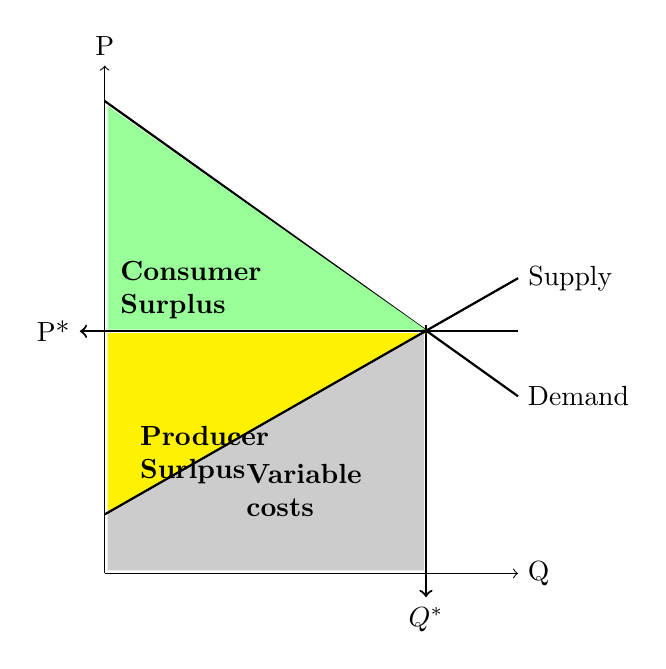
\begin{tikzpicture}[scale=1.5]
%\draw[thick,color=gray,step=.5cm, dashed] (-0.5,-.5) grid (3,3);
\draw[->] (0,0) -- (3.5,0) node[right ] {Q};
\draw[->] (0,0) -- (0,4.3) node [above] {P};
\draw[thick] (0,4) -- (3.5,1.5) ; \node [right]at (3.5, 1.5 ) {Demand}; 

\draw[thick,->] (2.72,2.1) -- (2.72,-.2) node[below] {$Q^*$};
\filldraw [color=green!40]  (0.03,2.07)-- (0.03,3.95)--(2.7,2.07)--cycle;
\filldraw [color=yellow] (0.03,2.03)-- (0.03,.515)--(2.7,2.03)--cycle;
\filldraw [color=gray!40](0.03,.515)--(2.7,2.03)-- (2.7,0.03)--(0.03,0.03)--cycle;
\draw[thick,<-] (-.21,2.05)node[left]{P*}  -- (3.5,2.05) node[above left] {}; 
%\fill[blue, opacity=.25]  (0,4) -- (1.86,2.1) --  (0,2.1) --cycle; 
%\fill[green] (0,.52) -- (1.82,2.1) --  (0,2.1) --cycle; 
\draw[thick] (0,.5) -- (3.5,2.5) node[right] {Supply};
\path (.7,2.4) node [text width=1.7cm](labelRent) {\textbf{Consumer\\ Surplus}};
\path (.8,1.) node [text width=1.5cm](labelRent) {\textbf{Producer\\ Surlpus}};
\path (1.7,.7) node [text width=1.5cm](labelvarcost){\textbf{Variable\\ costs}};
%\path (1.7,-1) node [black](labePC) {With producible capital};
  \end{tikzpicture}     
\caption{The basic supply and demand model determines price and quantity.}
\label{fig:Equilibrium}
\end{center}
\end{figure}


% \subsection{Another cliff}
% In neoclassical economics, however, the focus is on the exchange price and the marginal conditions satisfied in exchange, which neoclassical economics explains more satisfactorily than the classical approaches did.  

% %We do use their approach to distributing the distribution of the productive surplus to workers. - 

% Many of the cliffs neoclassical analysis runs off of are well understood. LIST. We propose another cliff. DESCRIBE.

% We can address one set of problems by re-introducing rent in the classical sense within an urban model. EXPLAIN.

% \section{ADD Neoclassical theories of production}


LINK 2 STORIES - RENT HAS PERSISTED, BUT A BIG GAP -WE BRING IT BACK TO FILL THE GAP


\subsection{The classical approach to rent in modern economic theory}

With the centrality  and the sucess of the neoclassical appraoch, with essentially a different underlying model of how the economy distirbutes surplus value, rent has played less of a central role.

Rent however remains absolutely central in modern ecnomic analysis. For instance ehre are a few examples.
% Econ has shifted away from rent, but it has persisted. 

% CORE IDEA PERSISTED INTO MODERN ECON - SEE MODERN EXAMPLES..
The classical idea of rent and rent has persisted and passed into modern economics in a number of forms. Several examples include: % ***E 

% MOVE DOWN suppressed as a concept as though it appears in a huge number of contexts, thought not under the name, but it appears not in the clasical
% drop land out of neoclaclasical analysis since were not focuse on fixed/unchangible factors

 % ADD BACK *** Modern economists generally focus  on the exchange price and the marginal conditions satisfied in exchange, which neoclassical economics explains more satisfactorily They appear to have abandoned rents as a central concept, but it  persists in slightly covert forms at the centre  neoclassical economics. 
\begin{enumerate}
    \item Alfred Marshall identified industrial profits as a form of rents, terming them `quasi-rents'' to emphasize that, unlike land rents, industrial profits would  be expected to disappear over time as new firms entered the industry.]
    \item First year students are taught that the high salaries of  sports stars are rents on their scarce talents. 
    \item First year students also learn about ``consumer surplus'' and ``producer surplus'' in supply and demand analysis. Both of these concepts are variants of rent and are essential in demonstrating the efficiency of a markets and the social losses due to monopoly, monopsony, regulation, and taxes. Consumer surplus is the sum of rents that accrue to the class of consumers (buyers). It is an inframarginal quantity, like land  rent, that accrues to the class of landowners. It arises because consumers have differing capacity to produce  utility with the good, just as landowners have lands with different abilities to produce agricultural output. Producer surplus corresponds precisely to land rent in Figure~\ref{fig-rent-ricardo}.  
    \item The First Fundamental Theorem of Welfare Economics, proven independently by Kenneth Arrow \cite{arrowExtensionBasicTheorems1951}and  Gerald Debreu \cite{debreuCoefficientResourceUtilization1951}  in 1951, possibly the most significant theorem in the social sciences,   demonstrates that perfectly competitive markets would maximize producer and consumer surplus, quantities that really are variants of rents.
    \item The ``\gls{bid-rent curve}'' became a dominant device  in urban theory with William Alonzo's 1961 thesis \cite{alonzoTheoryUrbanLand1960}, although the idea has deep roots and others were exploring the principle at the same time.  DEFINE BID RENT, LINK WITH REST OF THESIS.
    \item The theory of ``\gls{rent-seeking}''   became the subject of durable interest among economists and political scientists after the publication of two influential papers on the topic by Gordon Tullock in 1967 \cite{tullockWelfareCostsTariffs1967}, and Anne Krueger \cite{kruegerPoliticalEconomyRentSeeking1974} in 1974. Rent-seeking occurs when an someone seeks to increase their own wealth without creating any benefits or wealth to the society. Financialization, as we use the term, is a variety of rent-seeking
\end{enumerate}
% SHORT CLASSICAL EXAMPLE. Or, in a modern example, professional sports players' income, above the opportunity cost they could get working at another position, is rent they capture for their skill.

\section{Neoclassical production theory}
The \gls{neoclassical} approaches to economic analysis built on the classical framework. They added  mathematical modelling and the use of calculus. Calculus made it much easier to derive formal statements of what came to be called ``marginal conditions', or rules for efficient choice. It also allowed economists to derive clear rules for complex cases that were very difficult to state verbally. For example, the utilitarian goal of `the greatest good for the greatest number' which is comprehensible but vague could be translated into a guideline expressed in terms of the sums of individual marginal utilities equalling the marginal social cost for each good. 

%*E THIS PARAGRAPH SEEMS TO MOVE VERY FAST %i THINK YOU NEED TO EXPLIAN MARGINAL CONDITIONS IN MORE DETAIL, REALLY MAKE THAT CLEAR THEN BUILD OUT THE UTILITARIAN GOAL AS MORE OF A FLESHED OUT EXAMPLE. IT SEEMS LIKE THE SKELETON OF WHAT YOU NEED TO INTRODUCE THESE CONCEPTS CLEARLY IS HERE BUT NOT ENOUGH. 

The results of this new style are analytically more precise than the verbal statements they replace, and more easily communicated accurately for those with some mathematical skill. The approach also tend to lay bare the precise condition - the background assumptions- that must hold for results to be true. A cost of this progress is that economics became less accessible for many people. 

It is important to remember that neoclassical economics did not overthrow the insights of the classical economists. It provided increased precision and power, and it shifted attention from questions of class and distribution to deriving efficiency conditions. Economics became less a collection of great thoughts about the economy and more a mathematical edifice that embodied most of those thoughts in a rigorously consistent way and was the path to ever more arcane insights.
% *E WHILE THIS IS INTERESTING AS AN ACCOUNT OF THE RELATIONSHIP BETWEEN ECONOMICS AND THE PUBLIC, I'M NOT SURE HOW IT SETS UP WHERE YOU ARE GOING WITH THIS CHAPTER. CAN YOU BRING IT BACK TO RENT OR DISTRIBUTION, HOW THE NEW APPROACHES RELATE TO PROBLEMS YOU ARE LOOKING AT IN THIS THESIS?

% \section{Neoclassical production theory}
The concept of a production function used by the increasingly mathematical neoclassical economists and  the rapidly developing statistical techniques  naturally led to attempts to identify the precise \gls{functional form} that would describe the contributions of labour, capital, and income to output.
% *E COULD YOU FLESH THIS OUT, ADD EXAMPLES % ALSO MAYBE ADD WHAT WAS HAPPENING AT THE TIME, WHAT WERE THE PEOPLE LOOKING AT WHEN THEY STARTED TO APPLY THESE TOOLS TO THESE QUESTIONS. THIS MIGHT BE A GOOD PLACE TO REFERENCE BACK TO PREVIOUS PARTS ABOUT MARGINALISTS TO SET CONTEXT. 
 
\subsection{Classical rent theory using neoclassical notation}
Ricardo, for example, did not write down a formal production function as later \gls{neoclassical} theorists would,\footnote{He did generate numerical examples to demonstrate comparative advantage, and others, such as the physiocrats, von Th\"unen and Marx developed models still cited today, but these were not central for classical theorizing.} but his verbal production theory can be put in the notation neoclassical economists later developed. In modern notation, Ricardo's production model can be written: 
% *THIS IS CONFUSING DID YOU PUT IT IN THIS FORM OR DID THE MARGINALISTS. NOTE.. %JUST ABOVE YOU SAY THE MARGINALISTS STARTED TO DO THIS. iS THIS AN EXAMPLE? OR YOU DOING WHAT THEY ALSO DID? cLARIFY. OR THIS CONFUSION MIGHT JUST GO AWAY WHEN YOU FILL OUT MORE EXAMPLES ABOVE

\begin{equation} 
Y=F(K,L,N).
\label{eqn-production-ricardo}
\end{equation} 

where  $Y$ is output, $K$ is capital invested, $L$ is labour and $N$  is the natural resource land.\footnote{This makes it a three-factor model of production.  In principle any number of factors can be included.}  
Ricardo does not specify a functional form, but, %like mathematical neoclassical economists, 
he does assume diminishing returns to all factors. 

The  rent, $\mathcal{R}$, that the landlord receives is the total market value of the potatoes produced minus the cost of the capital employed in improving the land and the wage bill for the labour employed: 

\begin{equation} 
\mathcal{R}= PQ-rk-wl
\label{eqn-rent-ricardo}
\end{equation} 
Equation~\ref{eqn-rent-ricardo} makes it clear that the rent is a residual or a \gls{surplus}. The land is not paid for its services. The value of the land is the \gls{present discounted value} of the surplus it generates for the owner, that is what it would be worth paying now, to capture the future rents from that land.

Ricardo's analysis of rents  can be expressed by focusing only on land:

\begin{equation} 
Y=F(L,N).
\label{eqn-production-ricardo-2}
\end{equation} 
while most modern neoclassical treatments of production simplify by omitting land and emphasizing capital:\begin{equation} 
Y=F(K,L).
\label{eqn-production}
\end{equation}  
This makes sense for a number of reasons. The economy has shifted from agriculture to industry and the focus of economic theory has shifted to manufacturing processes.

%Furthermore, according to the Ricardian theory, rent is a surplus above cost. It does not, therefore enter into price. Land is a fixed factor for society as a whole that is not consumed in  the process of production.  Neoclassical treatments of production focus price determination based on the cost of the last unit used, the marginal  unit of input, while rents are generated on all of the inframarginal units, those units used earlier, which are more productive. The marginal unit of land generates no rents. In neoclassical analysis, the rents disappeared from view for this reason. This difference is at the heart of the distinction between classical and neoclassical economic theory. 
% #E this distinction is because of the actual structural difference in the societies? Also because of the differ tools? and apporaches? 

 %The Principles tells us that as cultivation is extended and exchange increases, profits fall while rents increase. 

Leaving land out, however, creates a problem in  the neoclassical growth theories we will examine below. John B. Davis \cite{davisRicardoTheoryProfit1993} noted that ``Questions arise, however, when one turns to exchange between a sector paying rent and one not.'' 
Under the assumption of perfectly competitive goods and factors markets as well as marginal productivity pricing of capital and labour, neoclassical growth requires technical change to be generated outside the model because there are no resources left to innovate if both factors of production are paid their marginal product.\footnote{This follows from Euler’s theorem: if, for a given level of technology $\bar A$ output Y is produced according to a \textbf{constant returns to scale} and twice continuously differentiable function of capital and labour $F(K, L, \bar A)$, Euler’s theorem implies that $F_K K + F_L L=Y$, where $F_i$ is the marginal product of factor $i$. Payments to  capital and labour take up the entire national product and no resources are left to finance the production of technology-improving innovations. are paid their marginal product.} 
If, however, land is reintroduced, as it must be in an urban model, there must be rents and there is therefore a surplus available for innovation.
\footnote{An alternative and common approach is to assume imperfect competition, which may be based on increasing returns to scale, in which case firms with market power may achieve a surplus. ``Although seldom modeled outside the monopolistic competition framework, market incompleteness and imperfect competition are central to the new growth theories'' (Gilles Duranton, Growth and imperfect competition on factor markets: Increasing returns and distribution, European Economic Review, 44-2, 2000, 255-280), Similarly, Sjak Smulders and Theo van de Klundert conclude that ``Growth is higher in a more concentrated market provided that market power of firms is not too high,'' (Imperfect competition, concentration and growth with firm-specific R \& D, European Economic Review, 39-1, 1995,139-160).}

\subsubsection{The Cobb-Douglas Production Function}

In 1928, mathematician Charles Cobb and Economist Paul Douglas came up with a specific and very convenient functional form \cite{cobbTheoryProduction1928}\footnote{The function had apparently previously been used by Knut Wicksell, Philip Wicksteed, and L\'eon Walras.} that captured much of what economists were talking about. The function is just a \gls{generalized arithmetic mean}:
 
 \[Y=AK^\alpha L^\beta\]
 where $A$ is a constant scale factor, now commonly called \gls{total factor productivity}. This function becomes the workhorse of neoclassical growth theory in the second half  of the 20th century. Our urban model is a direct heir to developments in neoclassical growth theory.
 
%The Cobb Douglas function has several convenient features. One is that the sum of the coefficents tells us the degree of returns to scale. If $\alpha+\beta = 1$, we have constant returns to scale,

%Another is that the coefficients of the factors, $\alpha$  and $\beta$ turn out to be the elasticities of output with respect to capital and labour respectively as well as the income share of the factor. These made it relatively easy for economists to combine national data on labour and capital stocks or income with output to test the model.

The Cobb–Douglas form was developed and almost immediately tested against statistical evidence in the USA by Cobb and Douglas between 1927–1947. It was  their widely circulated empirical work seems to have permanently associated this simple function with Cobb and Douglas for economists.


%I have not followed this track down to give references.

% ALSO Imperfect Competition and \gls{total factor productivity} Growth  AZZEDDINE M. AZZAM, ELENA LOPEZ and RIGOBERTO A. LOPEZ. Journal of Productivity Analysis. Vol. 22, No. 3 (November, 2004), pp. 173-184 (12 pages)

%Sjak Smulders and Theo van de Klundert.Imperfect competition, concentration and growth with firm-specific R & D European Economic Review. Volume 39, Issue 1, January 1995, Pages 139-160
% Duranton, Gilles (1997) Essays on growth: imperfect competition, labour supply and local public goods. PhD thesis, London School of Economics and Political Science.  http://etheses.lse.ac.uk/1471/1/U105715.pdf

%\footntoe{Alberto Bucci.  R&D, Imperfect Competition and Growth with Human Capital Accumulation, 2003. Scottish Journal of Political Economy. https://doi.org/10.1111/1467-9485.5004004. This paper studies the long-run consequences of imperfect competition on growth and the sectoral distribution of skills within an R&D-based growth model with human capital accumulation. We find that steady-state growth is driven only by incentives to accumulate skills. In the model imperfect competition has a positive growth effect, while influencing the allocation of human capital to the different economic activities employing this factor input. Contrary to general wisdom, the share of resources invested in R&D turns out not to be monotonically increasing in the product market power and its correlation with the equilibrium output growth rate is not unambiguous.}

%NOTE URBAN COMPETITION PROVIDES INCENTIVES TO UPGRADE SKILLS!!!


% Both the Solow (1956) growth model and its Ramsey–Cass–Koopmans counterpart featuring an endogenous saving rate (Ramsey, 1928; Cass, 1965; Koopmans, 1965) but treat technical change as purely exogenous. In fact, under the assumption of perfectly competitive goods and factors markets as well as marginal productivity pricing of capital and labour, neoclassical growth requires technical change to be generated outside the model because there are no resources left to innovate if both factors of production. 

% 
% assuming that technical progress is labour augmenting (Uzawa, 1961), we can rewrite the production function as $F(K, AL$), where $AL$ is a measure of labour in efficiency units, or effective workers. Let k = K/(AL). Then, output per effective worker is y =Y/(AL)=f (k). Population grows at the constant rate n > 0 and, as we will assume throughout the whole paper, capital does not depreciate. The steady state of the Solow model solves

% $\frac{f(k_{ss}}{k_{ss}} = \frac{n+g_A}{s}kss s$

% Journal of Economic Surveys (2017) Vol. 31, No. 5, pp. 1272–1303 \c ECONOMIC THEORIES 1275


Classical rent re-appears in neoclassical theory as `economic rent' (``a money payment made for a factor of production that is over and above the minimum payment to keep it in its present use,'')  as quasi-or pseudo-rents (non-equilibrium rents that will be competed away in a competitive equilibrium according to Marshall.\footnote{see Lewis Cecil 4 Rent Under the Assumption of Exhaustibility, Quarterly Journal of Economics, May, 1914, Vol. 28, No. 3 (May, 1914), pp. 466-489}),  as consumer  and producer surplus in supply and demand analysis,  as rent profiles or Pseudo-rent curves in urban theory, as a major concern on resource economics, and the theory of rent-seeking. Economic rent is a surplus insofar as its payment is not necessary to ensure a supply of a particular factor of production. 


% HOUSING RENT IN THE NATIONAL ACCOUNTS
%   Owner-occupied housing is included in Peersonal Consumption Expenditure because the National Income and Producgt Accounts (NIPAs) treat the owner-occupant as if it were a rental business, or in other words, a landlord renting to him or herself. That is, BEA imputes a value for the services of owner-occupied housing (space rent) based on the rents charged for similar tenant-occupied housing, and this value is included in GDP as part of personal consumption expenditures. This imputation is necessary in order for GDP to be invariant when housing units shift between tenant occupancy and owner occupancy.

%Ricardo  clearly understood and used the concept of diminishing marginal product. This shows in his use of the terms ``extensive margin'' and ``intensive margin'' to explain the income of the landowner. He focussed on the difference between the cost of production on a unit of land and the revenue generated. The landlord would rent out all the land which generated at least enough to pay all the costs. Anything in excess of the costs could be charged as land rent to a tenant farmer.

%Clearly in his model there are two basic productive factors, land and labour. The landlord  receives the surplus generated by the land and the rest of the value of production goes to labour. 
Recent urban models, on the other hand, tend to ignore the production process and consider the locational implications of land and transportation costs on the location of people. Wealth distribution is often ignored. 

% \subsection{Marginalist dis tribution}
% MARGINALIST DISTRIBUTION
% we've been paying some people less than the market wage so our profits our higher. this is what it would be if we paid everybody

% FOOTNOTE - RELATIONSHIP with marginalist distribution story ******** TODO Does the marginalist approach assume they are not exploited? Is it an experiment in examining the case where production is non-exploitative? 
% In a sense if labour gets the marginal value of their product, are they exploited. It's a matter of interpretation.  -It has an attraction 
%Clark tried to make an ethic of this. if everyone is being paid the marginal product of their labour. We know that's an efficient outcome. If it's efficient, is it also fair
%Is it possible someone's taking out an extra large fair. Yes. Not fair for simple classical reason that labour has been exploited in the past and that the current owner ship is a result of exploitation. The ownership of land introduces a kind of exploitation-- clearly exploitation if you claim that. 
%Lot's of marxists didn't like Henry George making it a locational question, they wanted to keep it located in the factory.
% You could - well what value did they create -- in line with those other-- could interpret.. 
%What is the average value, because every worker is not just marginal, they're also average/identical. What is the value created by the whole of the workforce. Should they be paid the marginal value or the average value of their work.
%
%The avg value -- declining.. 
%The demand for labour is declining--  
%Every infra marginal worker has been paid less than the avg contribution 
%Every infra marginal workers should - 
%every marginal worker should get the average wage.. that's fair.

%Get to the margin - that's what you pay.. that's what the next worker is worth to the firm. .. 5th' worker is paid more than the 10th. should it be averaged out and paid to all workers? paid to worker, or should the difference between top and the marginal goes to the firm- -- that's profit.. pay everyone the marginal value and keep the rest as profit.. 
%Effective labour has a higher marginal product.. - even higher - higher for the firm.. - but they don't have to pay the workers that... firms only have to pay enough to get their marginal individual cost down to the wage. The problem there is if they're making more profit they want to expand the workforce, but that wage only supports a certain size of city -- they've got off raise the wage a bit.. so they face an upward sloping supply curve for labour=-- that's why you know there's an equilibrium.. declining product and upward sloping supply so they cross.

%(all the profit you earn on the way could be redistributed)

\cite{arvidssonUrbanScalingLaws2023} find that cities’ tails are responsible for 36–80\% of the observed superlinearities across indicators. 


\section{Human capacity}
Change to neoclassical theory in economic tracked a change in the dominant mode of production, from primarily agricultural to primarily industrial.

We are now arguably in a third dominant mode of production, centered on  human capacity, (and computer/digital capacity). This is a new dominant mode of production but does not yet have a corresponding theory of distribution, and how that relates to production in space. 
This thesis works to fill that gap.\footnote{When a new dominant mode or age emerges, the old one doesn't go away. Stone work and bronze work still persist, agriculture and industrial production still persist, they are not however the force driving economic and social relations in the way the were when they were dominant as technologies and modes of production\cite{oldworldsdon'tdie}}
 
\section{Summary}
We have examined the main stages of rent and distribution theory
% as  a bridge from classical rent theory to the
as the necessary background for our development %extension 
of a modern theory of urban rent. On the way we explained how the concept of economic rent arises in an agricultural economy, and who gets the rents in that type of economy. We then gave an account of how rent theory and the classical distribution theory was pushed into the background as neoclassical theorists analysed the industrial market economy that emerged after the industrial revolution, and introduced modern theories of production. In the next chapter we introduce 20$^{th}$ century urban models that are essentially an application of classical rent theory.


What we do in our  model is essentially these two stories of the distribution of the surplus, the rents, together in one model, in the urban economy, to take advantage of the strengths of both approaches, and make a model of %making and taking
urban production of value based on human capacity in cities with agglomeration effects. 
This brings the essentially spatial models of finance together with spatial models of urban rents, to model the effects of financialization. 

and makes it possible to talk formally in the neoclassical tradition with foundational questions of distribution, and with the older traditions of classical economics. 


% The distribution of rents in the urban model affects urban productivity in our model.
%***E FINANCIALIZATION IS ABOUT SURPLUS. CURRENT THINKING ABOUT FINANCIALIZATION HAS NOT BEEN NOT BEEN PUT INTO A FORMAL MODEL. FORMAL MODELS COME FROM COME FROM THE NEO-CLASSICAL TRADITION. 